% ------------------------------------------------------------------------------
% Slide 2: El Mapa Acústico: Tres Puntos Cardinales y Vocales Intermedias
% ------------------------------------------------------------------------------
\begin{frame}{El Mapa Acústico: Tres Puntos Cardinales y Vocales Intermedias}
    \begin{columns}[c]
        \begin{column}{0.45\textwidth}
            \scriptsize
            \begin{block}{Topología en el Espacio de Formantes}
                Al proyectar las fonaciones en el plano espectral $F_1$ versus $(F_1 - F_2)$, la geometría articulatoria define un \textbf{triángulo vocal}:
                \begin{itemize}\setlength{\itemsep}{1pt}\setlength{\parskip}{0pt}
                    \item \textbf{Polos cardinales extremos:} Tres vértices fijos dados por \textbf{/a/}, \textbf{/i/} y \textbf{/u/}.
                    \item \textbf{Vocales intermedias:} Tanto la \textbf{/e/} como la \textbf{/o/} son estados físicos de transición a lo largo de las aristas del triángulo.
                \end{itemize}
            \end{block}
            \vspace{0.04cm}
            \begin{alertblock}{El Desafío Experimental de Sensado}
                \begin{itemize}\setlength{\itemsep}{1pt}\setlength{\parskip}{0pt}
                    \item Cada polo cardinal exige una configuración geométrica límite del tracto acústico.
                    \item \textbf{Pregunta de investigación:} ¿Cómo mapeamos de forma unívoca estos tres polos extremos utilizando únicamente tres canales de electromiografía de superficie?
                \end{itemize}
            \end{alertblock}
        \end{column}
        \begin{column}{0.53\textwidth}
            \centering
            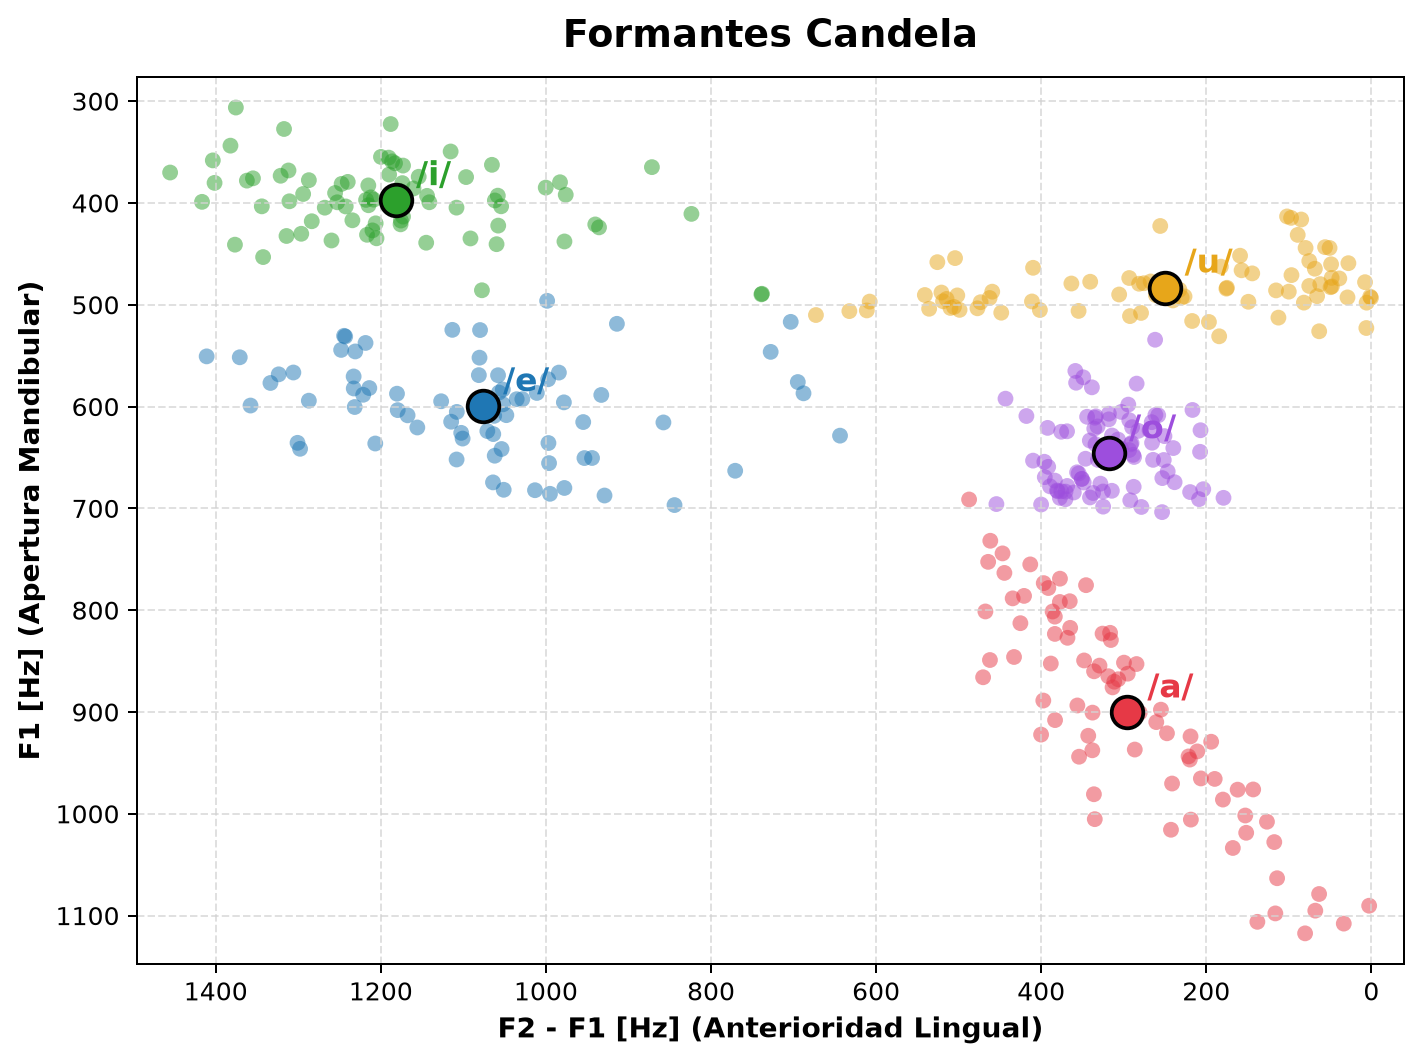
\includegraphics[width=\linewidth,height=0.37\textheight,keepaspectratio]{figuras/formantes_candela.png}\\[4pt]
            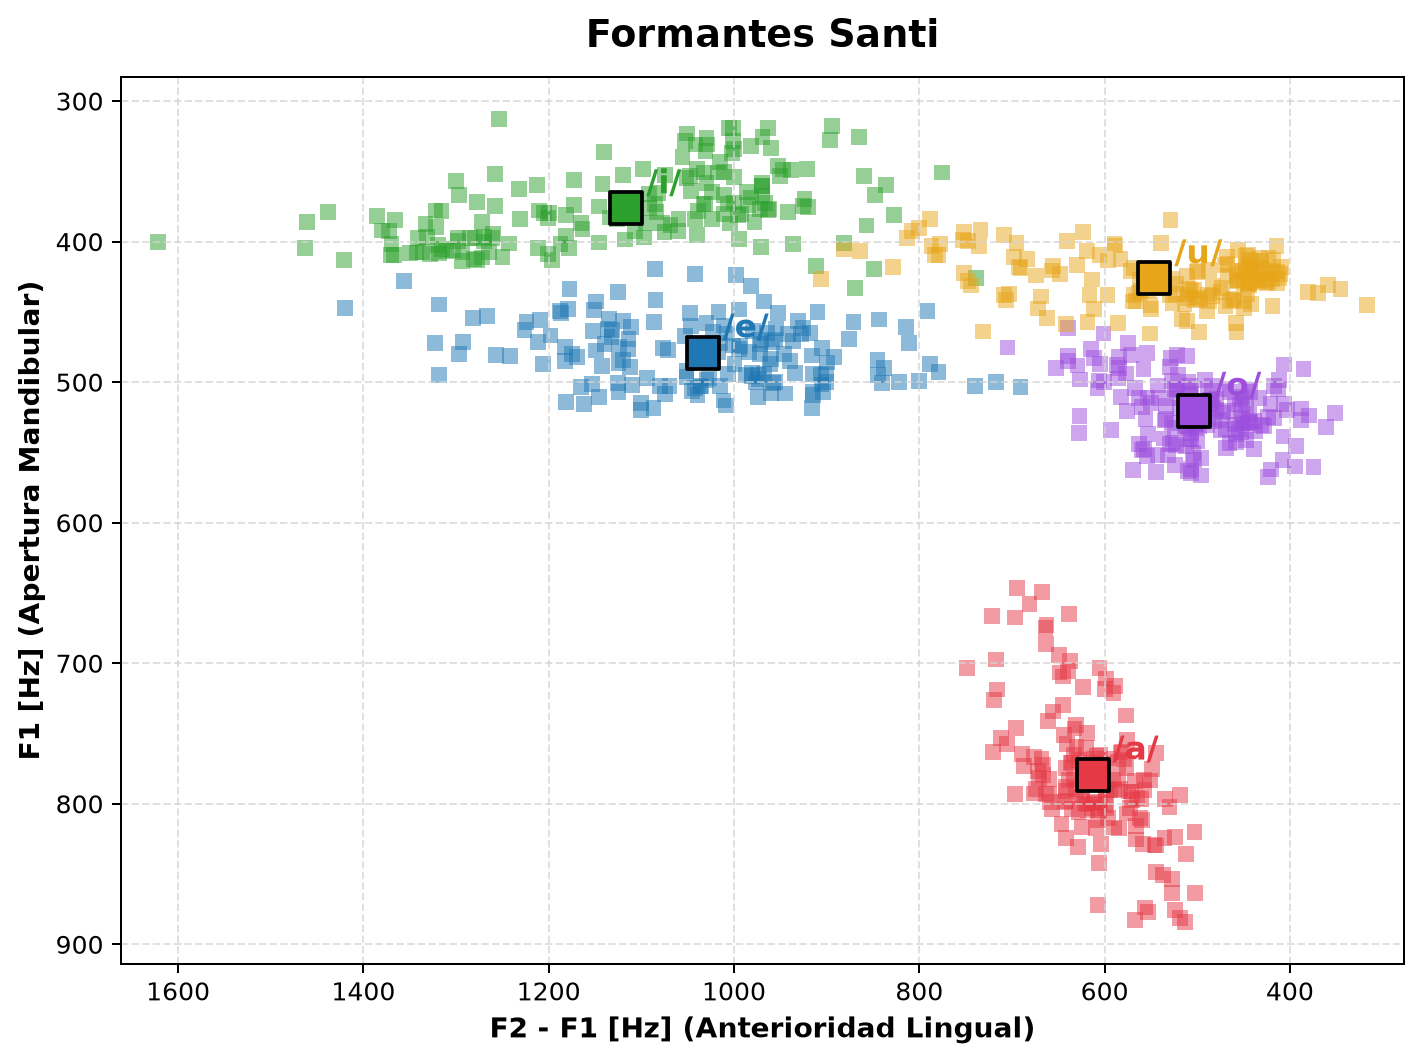
\includegraphics[width=\linewidth,height=0.37\textheight,keepaspectratio]{figuras/formantes_santi.png}
        \end{column}
    \end{columns}
\end{frame}
